
\documentclass[11pt]{article}
\usepackage[margin=1in]{geometry}
\usepackage{amsmath,amssymb}
\usepackage{booktabs}
\usepackage{tabularx}
\usepackage{graphicx}
\usepackage{float}
\usepackage[numbers]{natbib}
\title{Latent-Mixture-Induced Marginal NPH: A Full-Grid Simulation Comparison of Survival Methods}
\author{NPH Project}
\date{\today}
\begin{document}
\maketitle

\begin{abstract}
We evaluate common two-arm survival comparison methods under non-proportional hazards induced by latent subgroup mixture. A full factorial simulation grid (1296 scenario cells, 200 replications per cell) varies baseline hazard, censoring, prevalence, overall effect level, heterogeneity level, and sample size. To support inferential calibration, we add a strict-null benchmark (2000 replications per scenario). Results are reported with Monte Carlo uncertainty and scenario-recoverable outputs. Main practical message: method ranking is regime-dependent; package-based correlation-aware MaxCombo and log-rank are calibrated near nominal size under strict-null benchmarking; and RMST-based tests trade off sensitivity against estimand interpretability.
\end{abstract}

\section{Introduction}
When biomarker heterogeneity exists but the biomarker is not used in primary analysis, treatment-arm survival may exhibit marginal non-proportional hazards (NPH) even if subgroup hazards are proportional. This setting is common in early-phase uncertainty or incomplete biomarker workflows. Our scientific target is the \emph{marginal overall treatment comparison} (not subgroup effect estimation). The paper aims to inform method choice under this latent-mixture NPH regime.

Methodological options for NPH are broad: weighted log-rank families and related FH classes \citep{harrington1982,fleming1991,magirr2019}, correlation-aware MaxCombo combinations \citep{ristl2021}, RMST-based estimands and tests \citep{uno2014,cho2021}, weighted Cox/average hazard ratio formulations \citep{schemper2009}, and flexible parametric survival modeling alternatives \citep{royston2002}. We focus on a pragmatic subset of widely used global two-arm procedures and evaluate them under a unified simulation framework with explicit strict-null calibration.

\section{Methods}
\subsection{Data-generating process and parameter mapping}
Biomarker prevalence levels were 0.1, 0.3, and 0.5. Control hazard levels (per month) were $\log(2)/36$, $\log(2)/12$, and $\log(2)/6$. Total sample sizes were 300, 500, 1000, and 1500 (1:1 randomization). Treatment subgroup hazards are parameterized by
\begin{align}
HR_+ &= HR_{overall}\times r, \\
HR_- &= \frac{HR_{overall}-p\,HR_+}{1-p},
\end{align}
where $HR_{overall}\in\{1.0,0.9,0.8,0.7\}$ and heterogeneity level $r\in\{0.9,0.8,0.7\}$.
Thus $p\,HR_+ + (1-p)\,HR_- = HR_{overall}$, where $HR_{overall}$ is a \emph{design control parameter} (not a marginal causal estimand).

Control and treatment survival are
\begin{align}
S_0(t)&=\exp(-\lambda_0 t), \\
S_1(t)&=p\exp(-\lambda_0 HR_+ t)+(1-p)\exp(-\lambda_0 HR_- t).
\end{align}
This induces marginal NPH via mixture.

\subsection{Censoring and follow-up}
Independent exponential censoring is used:
\begin{align}
C\sim \mathrm{Exp}(\lambda_C), \qquad \lambda_C=\frac{c}{1-c}\lambda_0,
\end{align}
with target levels $c\in\{0,0.1,0.3\}$. No accrual or administrative cutoff is imposed in the main grid. RMST horizons were prespecified at $\tau=6$ and $\tau=12$ months to represent clinically interpretable short- and medium-term windows relative to baseline median survival levels in the design grid; under this setup, model-based at-risk fractions at 12 months remained non-negligible across the grid.

\subsection{Methods, hypotheses, and implementation details}
All tests are two-sided with nominal $\alpha=0.05$.
\begin{itemize}
  \item Log-rank: \texttt{survival::survdiff} chi-square p-value (1 df).
  \item FH weighted log-rank: pooled KM weights $w(t)=\hat S(t)^\rho(1-\hat S(t))^\gamma$ \citep{harrington1982,magirr2019}. Weight pairs used: $(0,0)$, $(0,1)$, $(1,1)$, and $(1,0)$. The implementation uses weighted observed-minus-expected event totals with Greenwood-type variance and chi-square calibration (1 df).
  \item MaxCombo (primary): correlation-aware implementation via \texttt{nph::logrank.maxtest} with FH weights $(0,0)$, $(0,1)$, $(1,1)$, and $(1,0)$; the primary p-value is the multiplicity-adjusted \texttt{pmult} from the joint covariance-based combination \citep{ristl2021}.
  \item Optional reference: Bonferroni minimum-$p$ over the same four FH components is reported when available as a conservative sensitivity benchmark (not the primary decision rule).
  \item Cox PH: \texttt{survival::coxph} Wald p-value with Efron ties \citep{cox1972}.
  \item RMST tests: \texttt{survRM2::rmst2} unadjusted two-group comparison at $\tau\in\{6,12\}$ \citep{uno2014,cho2021}.
\end{itemize}

\paragraph{On estimands.}
RMST effects target $\Delta_R(\tau)=\int_0^\tau(S_1-S_0)$. Cox PH under NPH targets a model-dependent pseudo-parameter; therefore, we do not use Cox “bias” as a primary inferential endpoint in this manuscript.

\subsection{Monte Carlo uncertainty}
With $R=200$ per grid cell,
\begin{align}
MCSE(\hat p)=\sqrt{\hat p(1-\hat p)/R}.
\end{align}
For bias summaries, $MCSE(\widehat{bias})=\sqrt{\max(MSE-bias^2,0)/R}$.

\subsection{Protocol coverage and recoverability}
The grid has $3\times3\times3\times4\times3\times4=1296$ cells. Each cell has deterministic \texttt{scenario\_id}. Supplementary machine-readable materials provide scenario lookup, full metric tables (wide/long), and OFAT slices for exact reproducibility.

\section{Results}
\subsection{DGP diagnostics and NPH severity}
\begin{figure}[H]
\centering
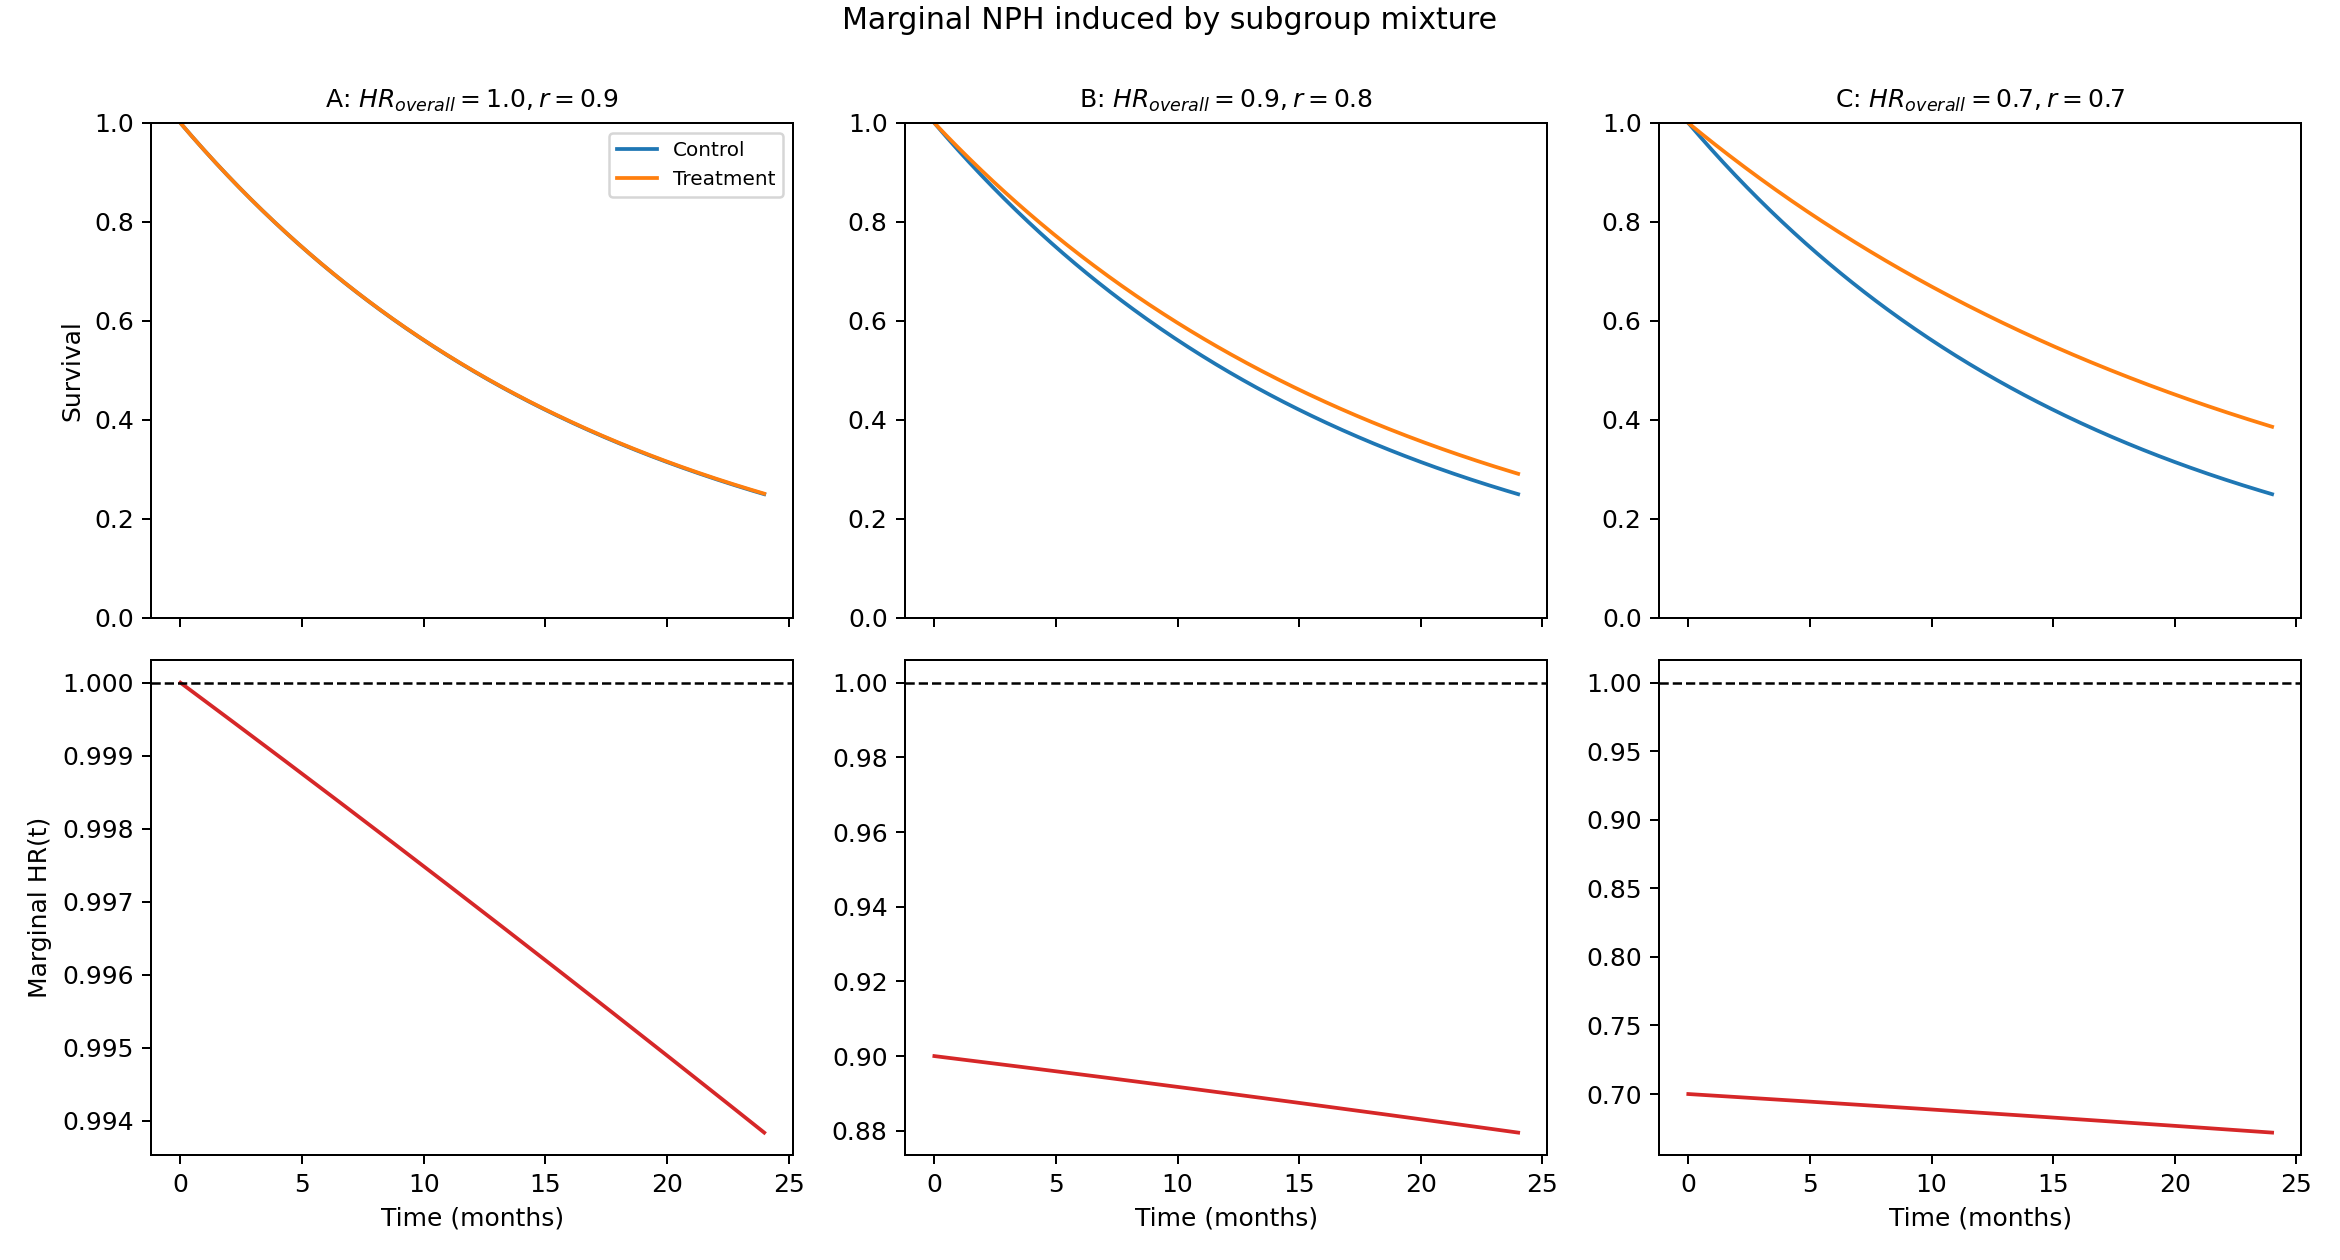
\includegraphics[width=0.98\textwidth]{figures_protocol_full/fig1_dgp_sanity.png}
\caption{Representative scenarios: survival curves (top) and implied marginal $HR(t)$ (bottom).}
\end{figure}

In alternative cells, the NPH-severity index $\max_t HR(t)-\min_t HR(t)$ had 10th and 90th percentiles 0.0013 and 0.0667, respectively.


\subsection{Strict-null size benchmark}
To address strict type-I-error questions, we ran an additional benchmark under $HR_+=HR_-=1$ (true equal-survival null), using 6 representative scenarios and 2000 replications per scenario.
Across primary methods, mean strict-null rejection was 0.0523 (log-rank), 0.0515 (MaxCombo), and 0.0503 (RMST12), all close to nominal 0.05 within Monte Carlo uncertainty.

\begin{figure}[H]
\centering
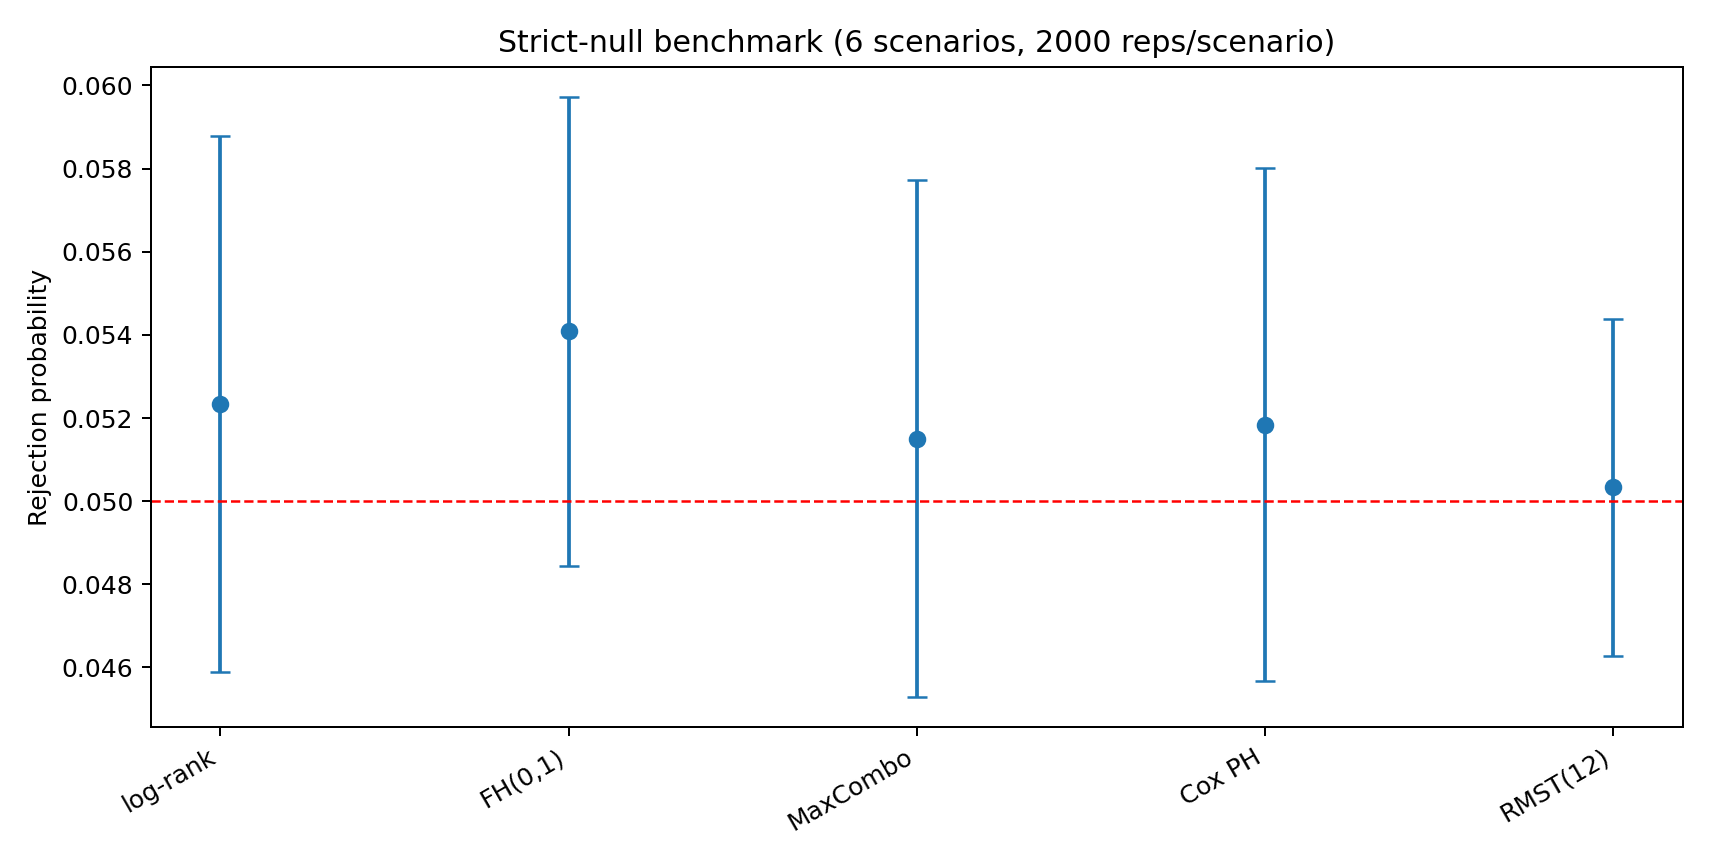
\includegraphics[width=0.88\textwidth]{figures_protocol_full/fig2_strict_null_size.png}
\caption{Strict-null benchmark across methods (mean and between-scenario variability over 6 strict-null scenarios).}
\end{figure}

\begin{table}[H]
\centering
\small
\begin{tabular}{lrr}
\toprule
Method & Mean strict-null rejection & Worst-case strict-null rejection \\
\midrule
log-rank & 0.0523 & 0.0605 \\
FH(0,1) & 0.0541 & 0.0605 \\
MaxCombo & 0.0515 & 0.0585 \\
Cox PH & 0.0518 & 0.0600 \\
RMST(12) & 0.0503 & 0.0540 \\
\bottomrule
\end{tabular}
\caption{Strict-null size benchmark summary (2000 reps/scenario).}
\end{table}

\begin{table}[H]
\centering
\small
\begin{tabular}{rrrr}
\toprule
Target censoring level & Mean realized censoring & Arm 0 censoring & Arm 1 censoring \\
\midrule
0.1 & 0.100 & 0.100 & 0.100 \\
0.3 & 0.300 & 0.300 & 0.299 \\
\bottomrule
\end{tabular}
\caption{Realized censoring in strict-null benchmark scenarios.}
\end{table}


\subsection{Power across alternative cells}
\begin{figure}[H]
\centering
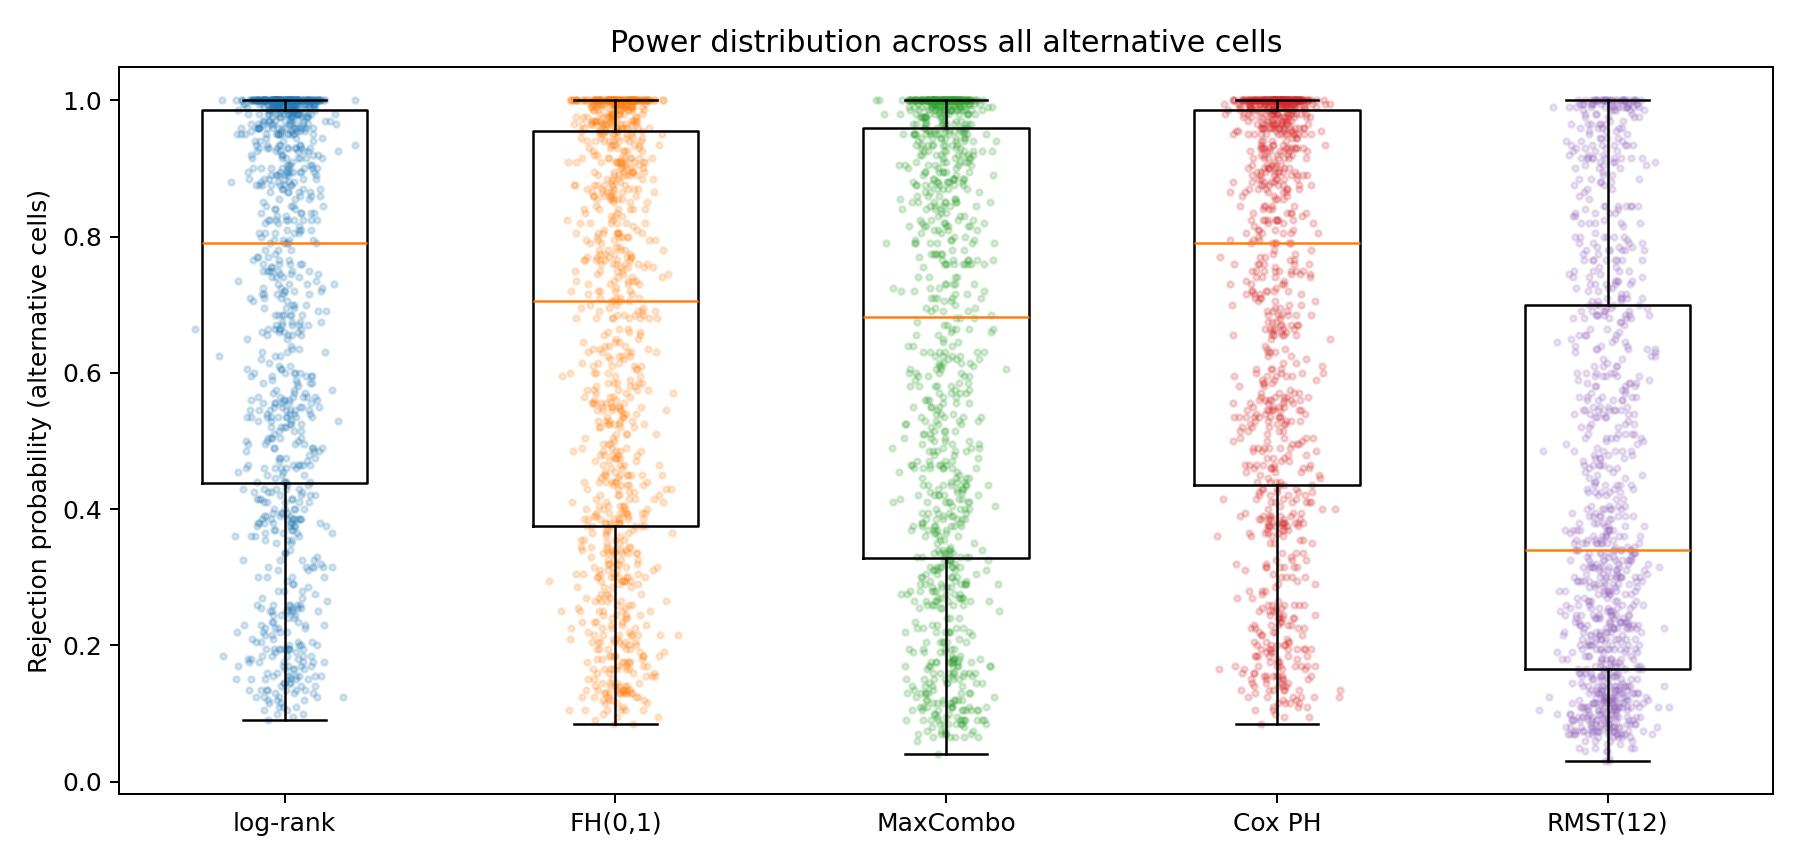
\includegraphics[width=0.9\textwidth]{figures_protocol_full/fig3_power_boxplot.png}
\caption{Power distributions across alternative cells ($HR_{overall}<1$).}
\end{figure}

\begin{figure}[H]
\centering
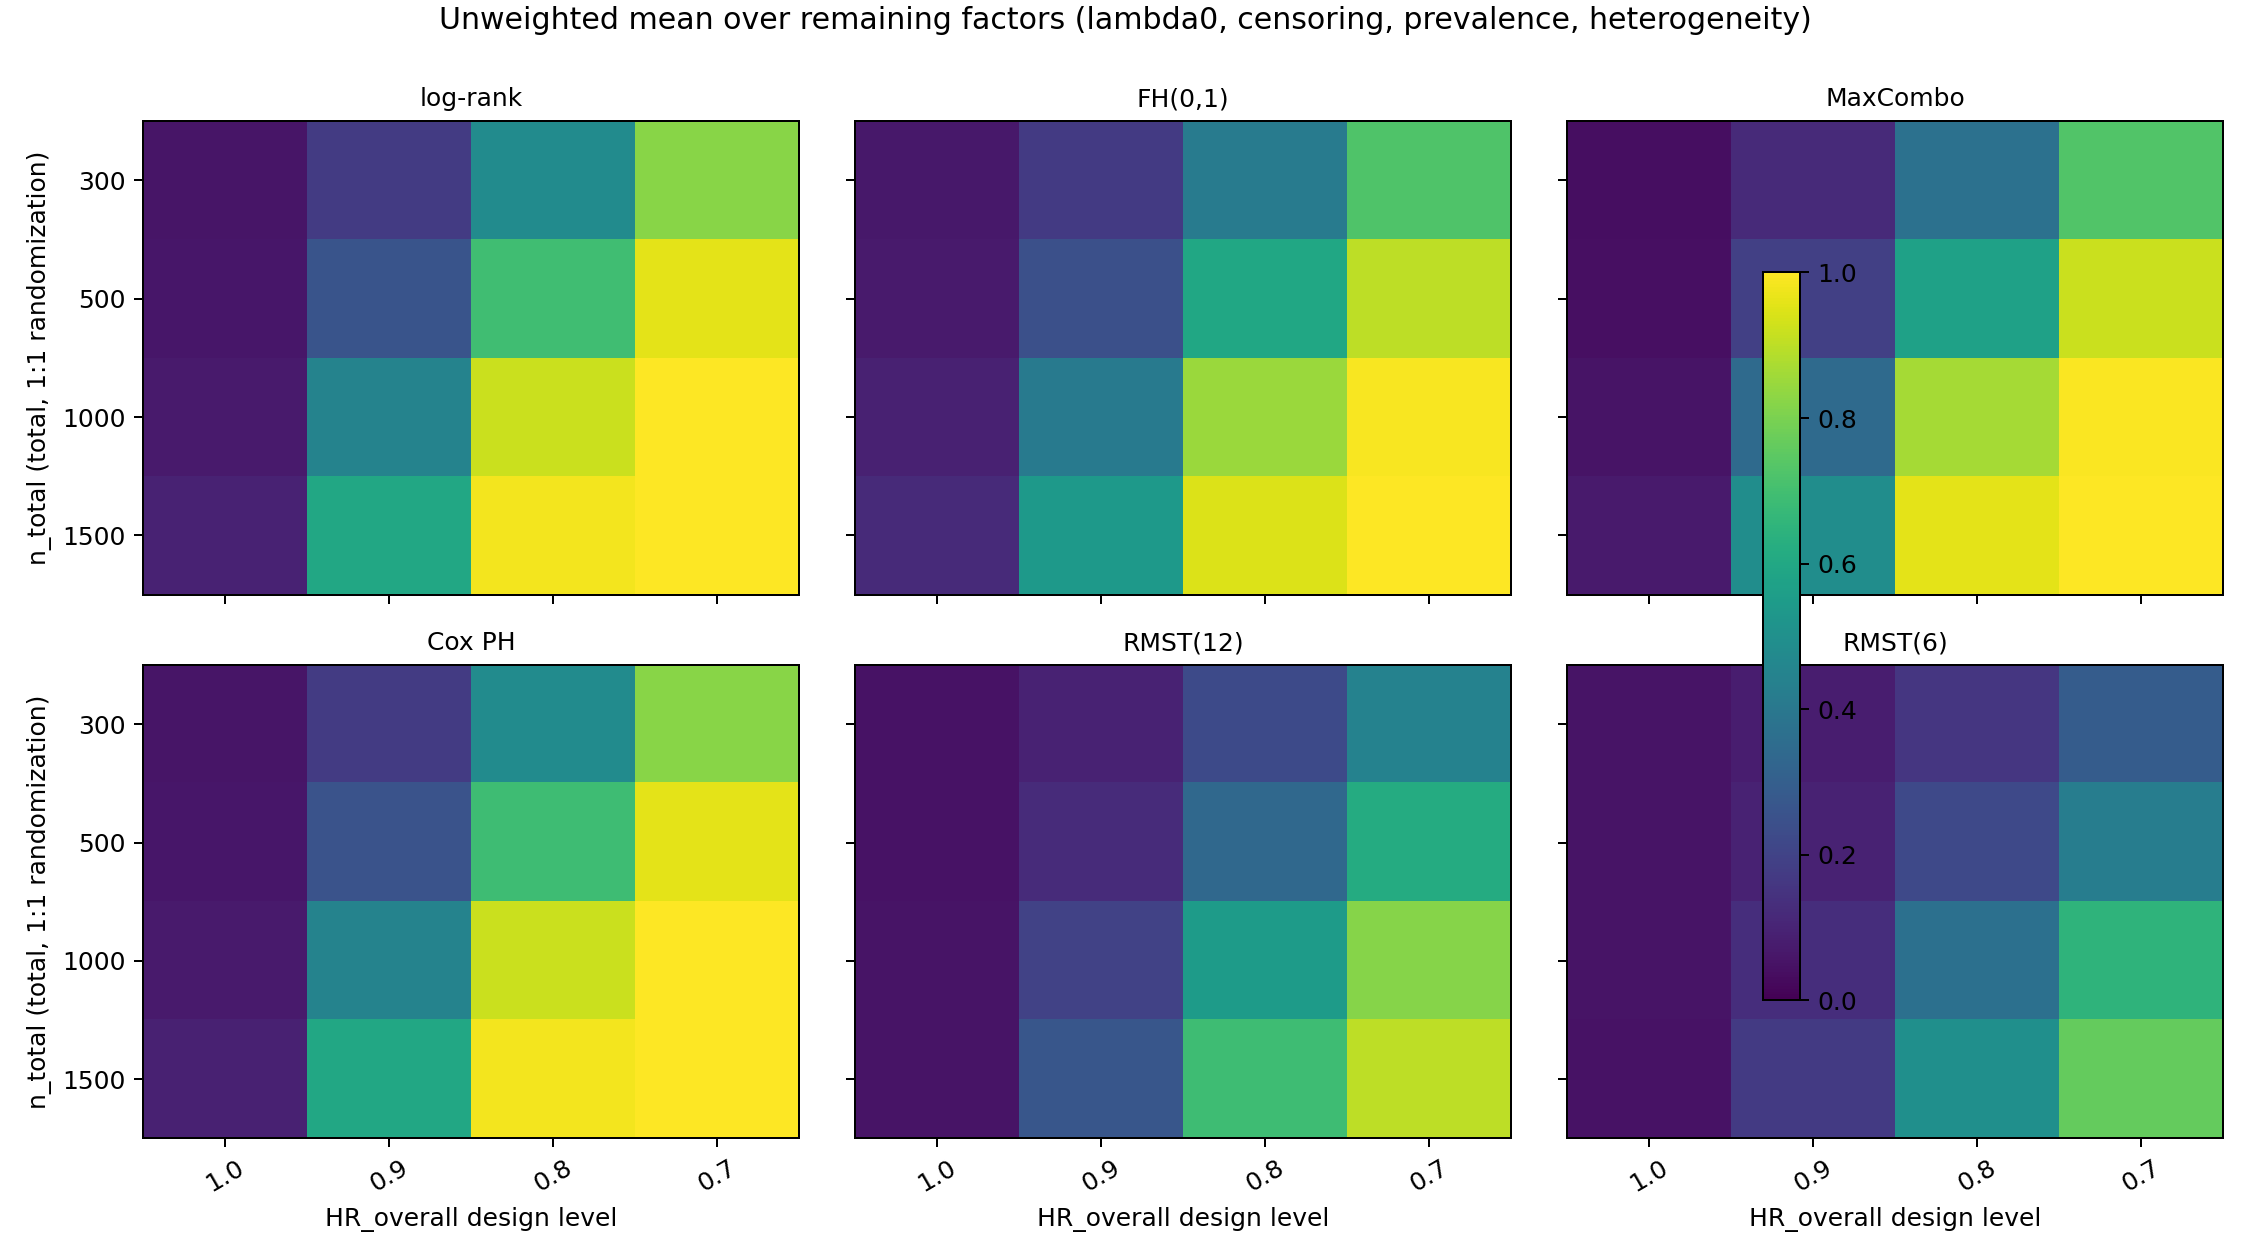
\includegraphics[width=0.98\textwidth]{figures_protocol_full/fig4_heatmap_methods.png}
\caption{Method-specific mean rejection on $(n_{total}, HR_{overall})$ grid, averaged uniformly over $(\lambda_0, c, p, r)$.}
\end{figure}

\begin{figure}[H]
\centering
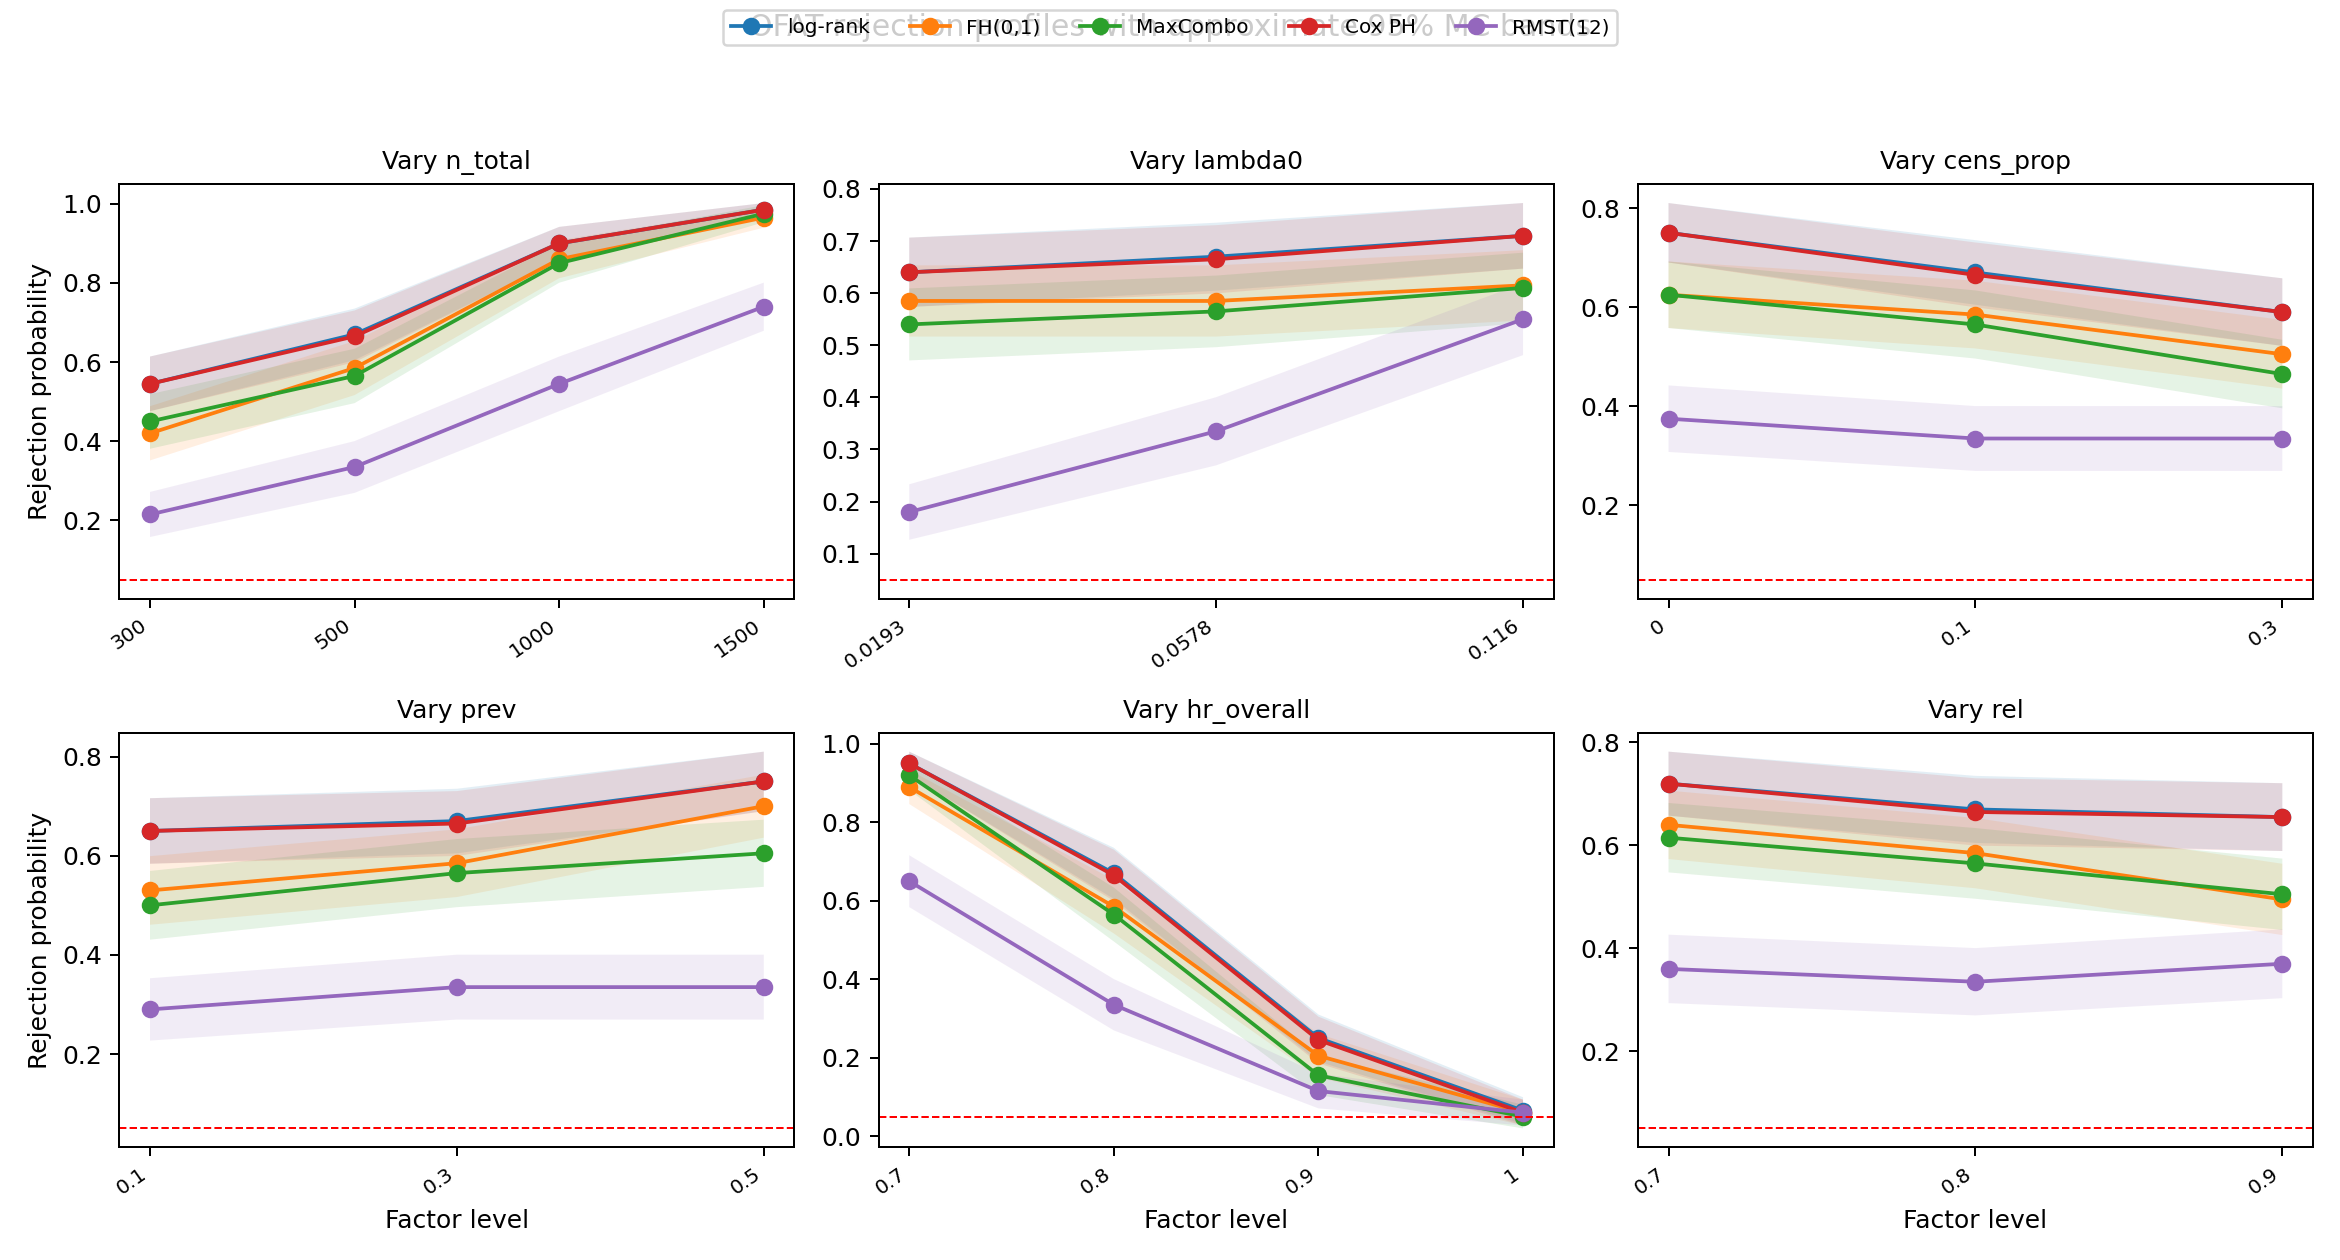
\includegraphics[width=0.98\textwidth]{figures_protocol_full/fig5_ofat_rejection_mcse.png}
\caption{OFAT rejection profiles around reference scenario ($n=500$, $\lambda_0=\log(2)/12$, $c=0.1$, $p=0.3$, $HR_{overall}=0.8$, $r=0.8$).}
\end{figure}

\begin{figure}[H]
\centering
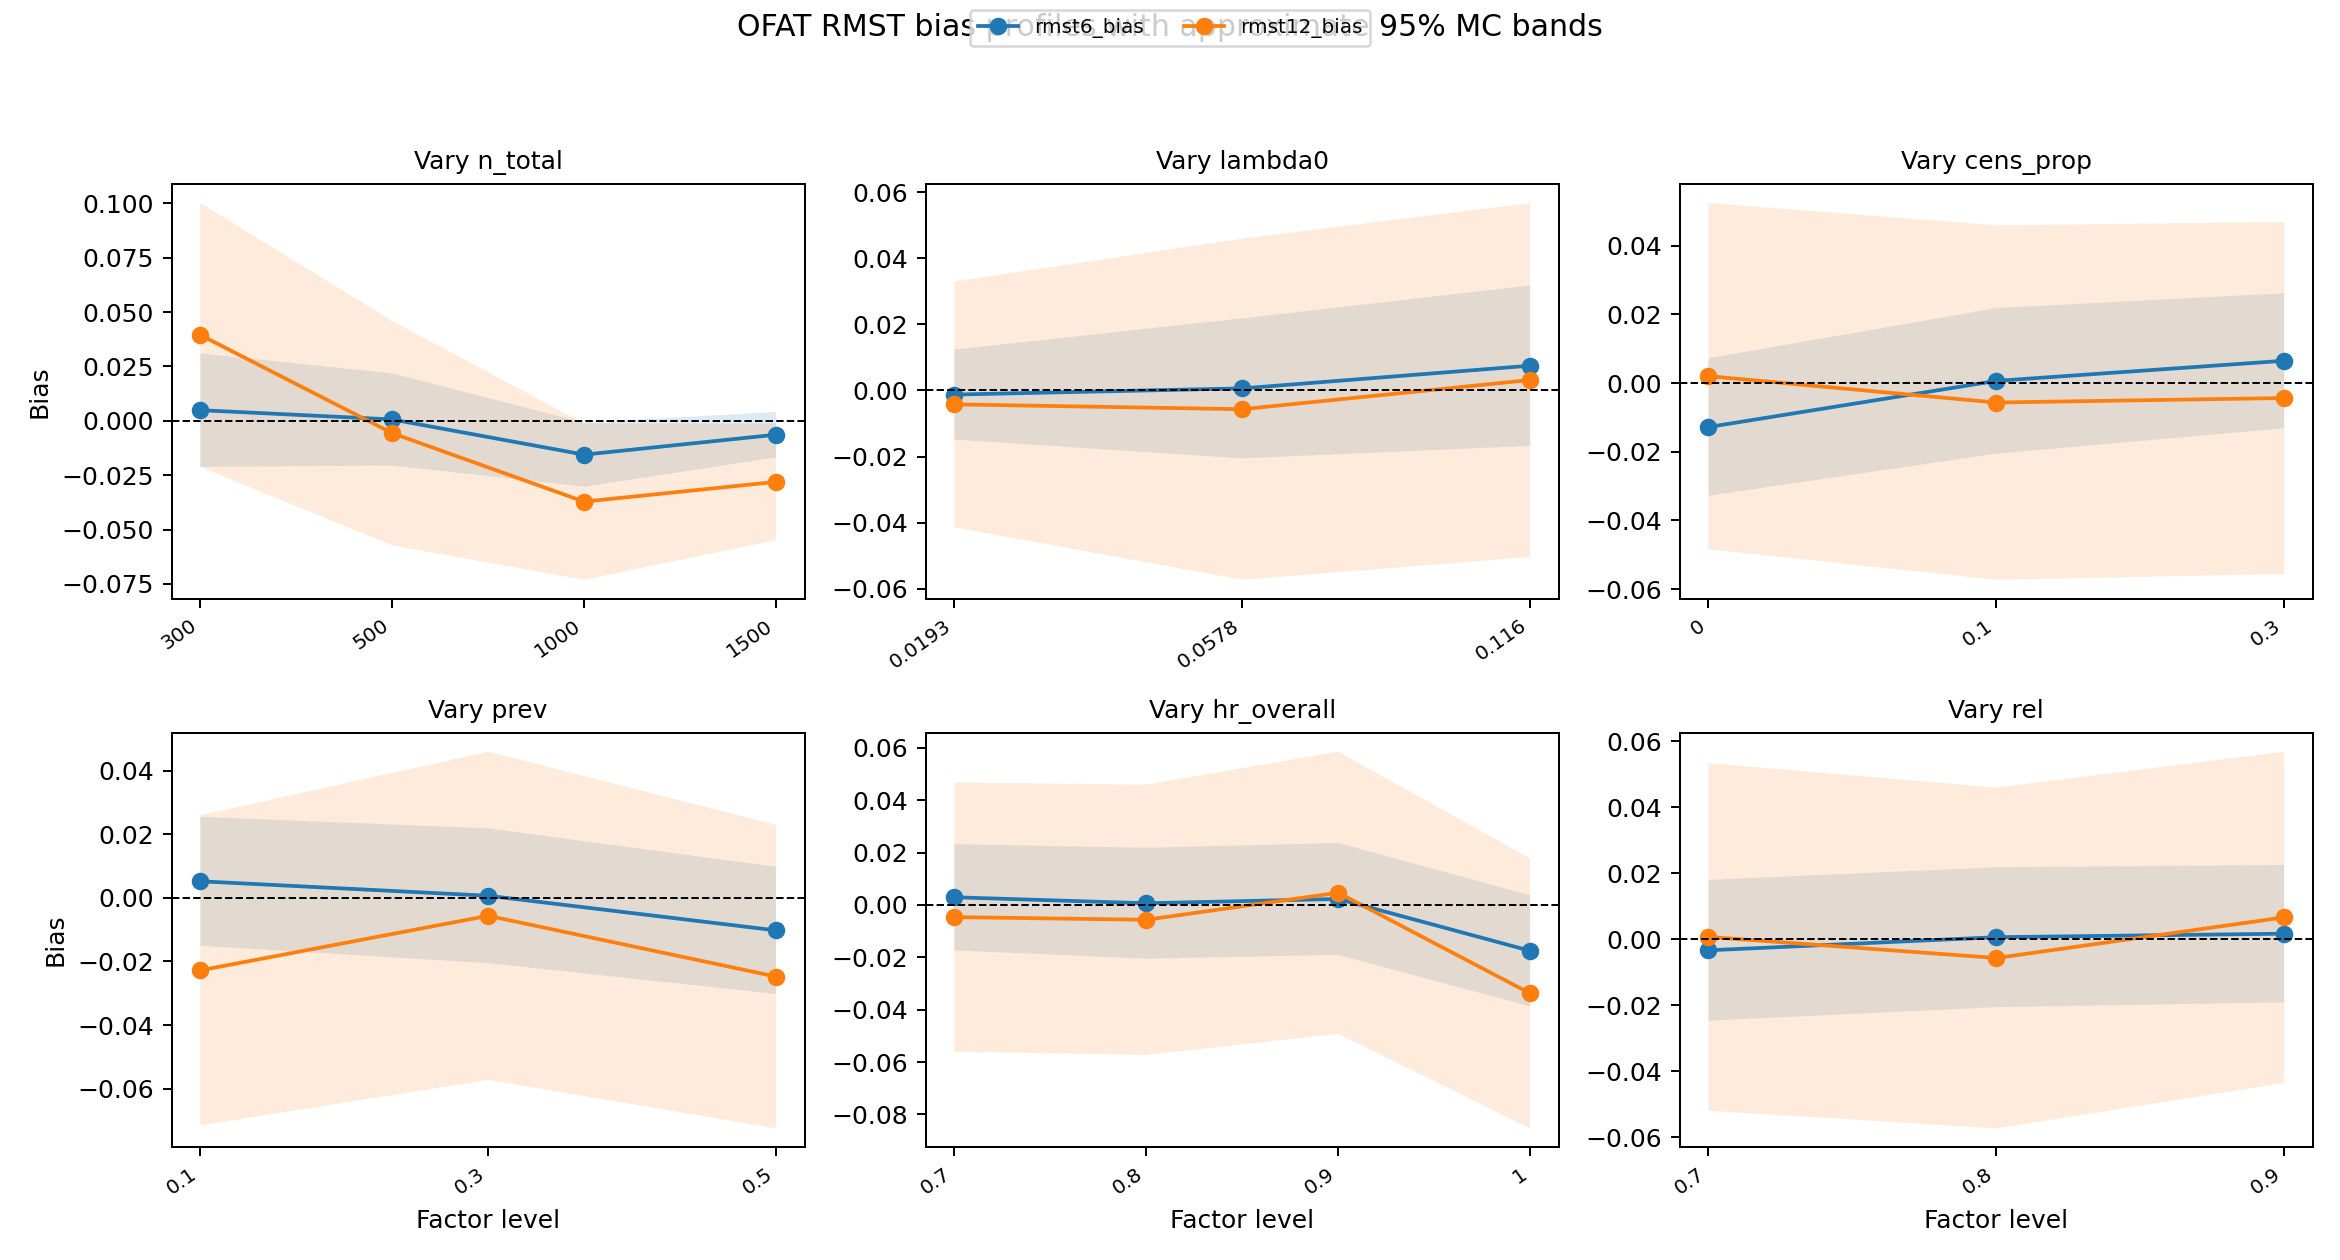
\includegraphics[width=0.98\textwidth]{figures_protocol_full/fig6_ofat_bias_mcse.png}
\caption{OFAT RMST bias profiles with MC uncertainty.}
\end{figure}

\begin{figure}[H]
\centering
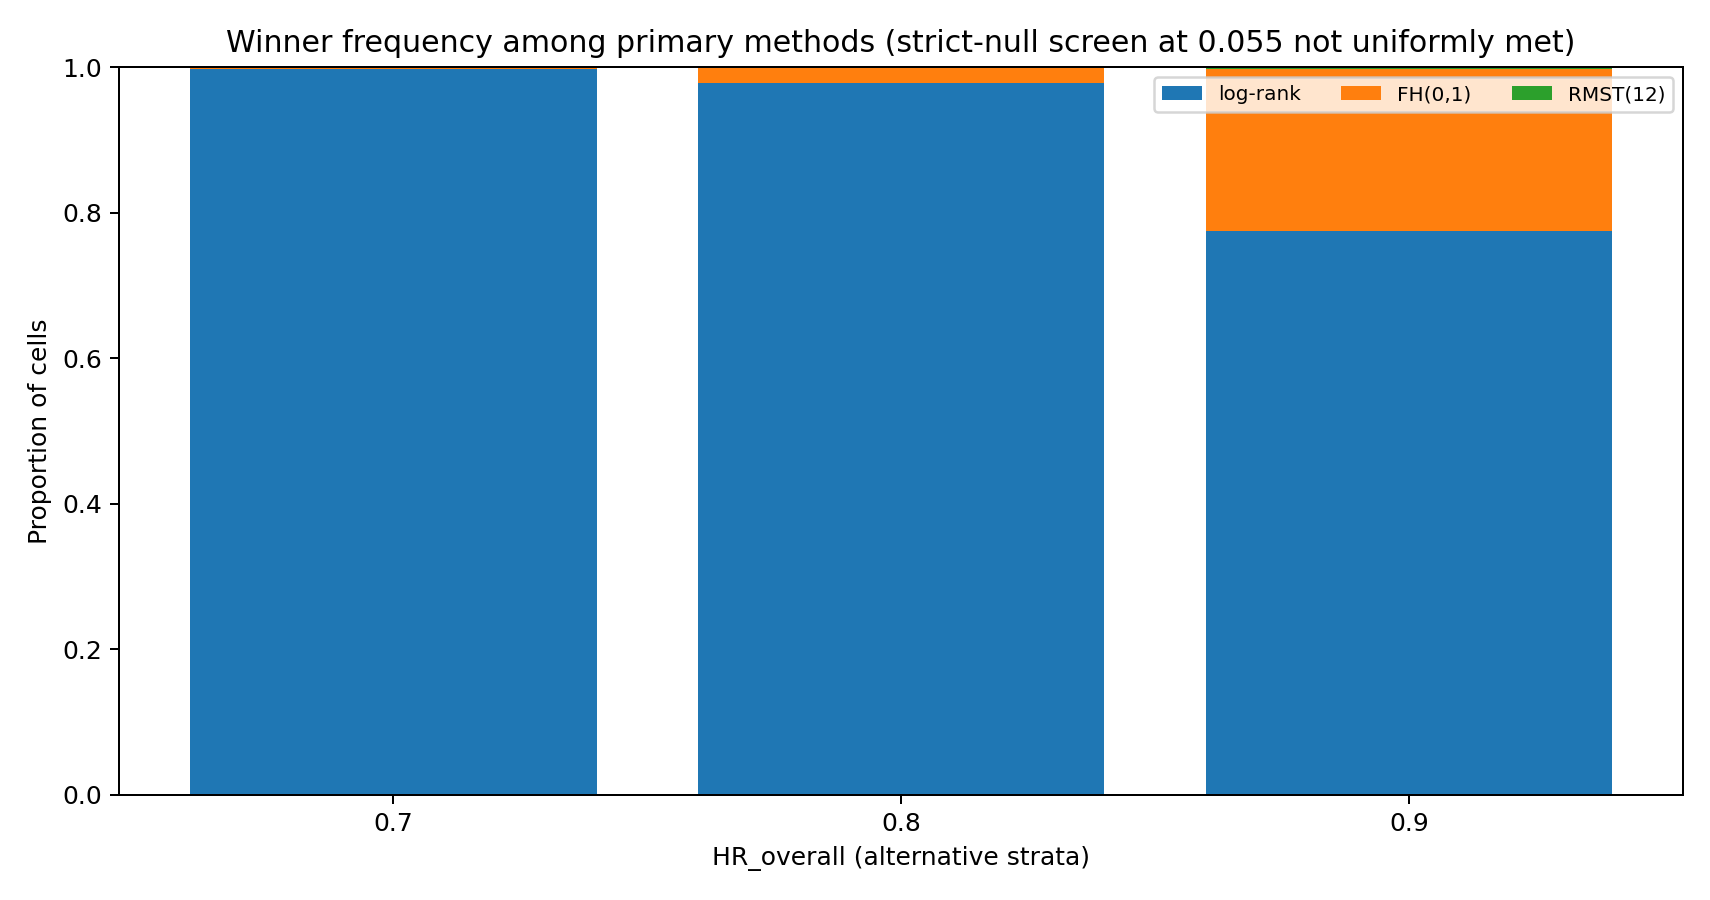
\includegraphics[width=0.85\textwidth]{figures_protocol_full/fig7_winner_frequency.png}
\caption{Winner frequency among primary methods. A strict-null screen at 0.055 was not applied because at least one primary method exceeded the threshold.}
\end{figure}

\begin{figure}[H]
\centering
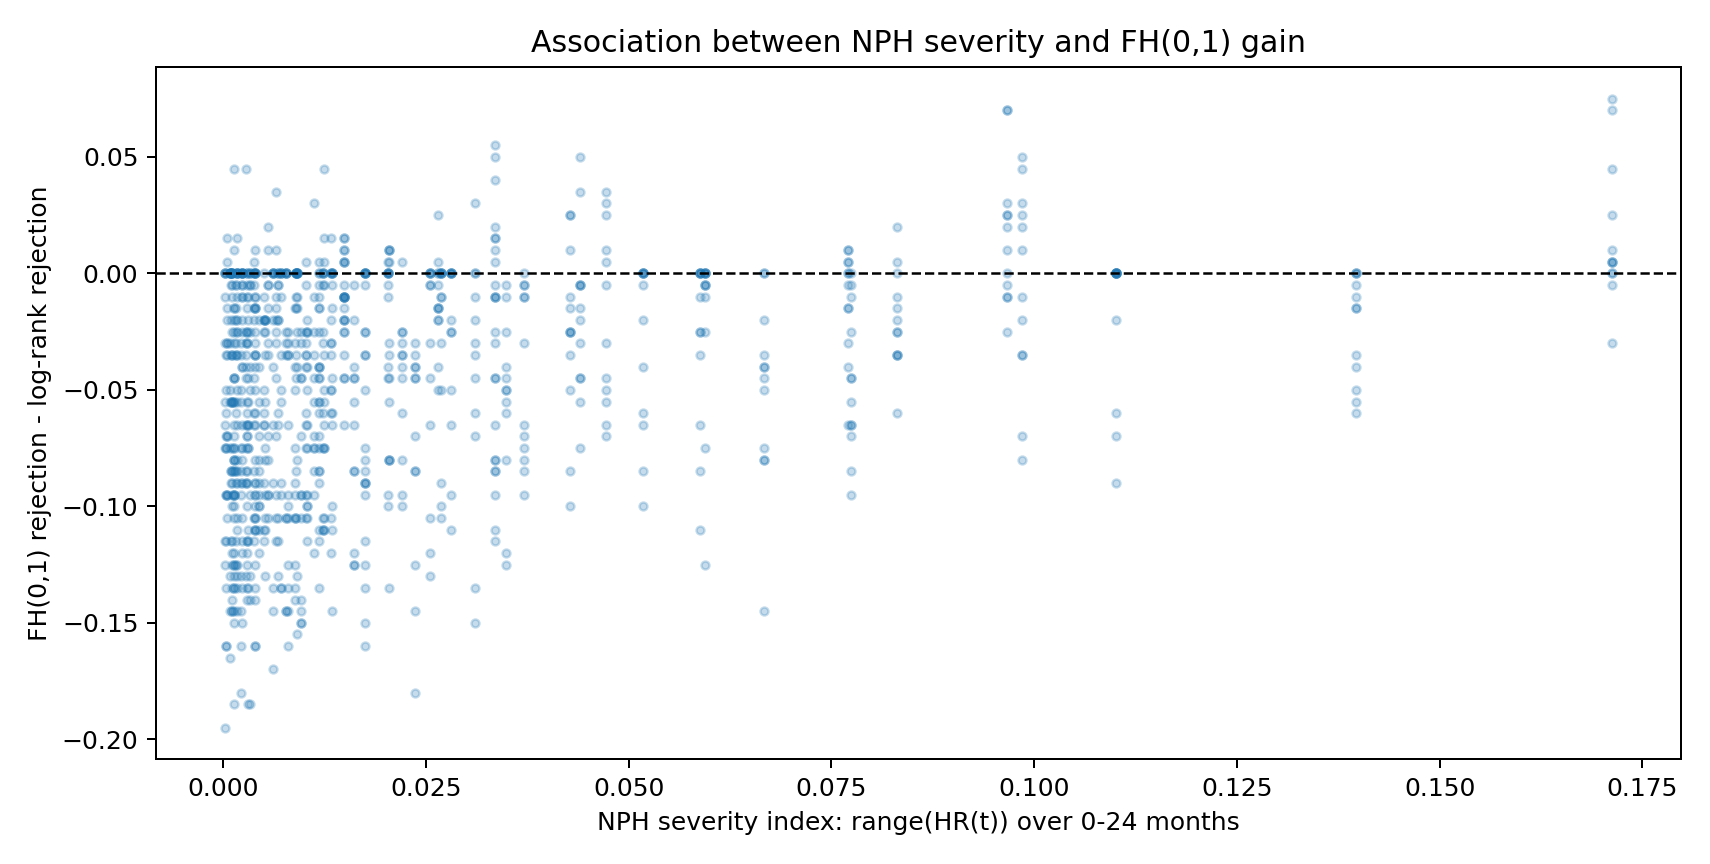
\includegraphics[width=0.9\textwidth]{figures_protocol_full/fig8_nph_gain_scatter.png}
\caption{FH(0,1) gain vs log-rank as a function of NPH-severity index.}
\end{figure}

\begin{table}[H]
\centering
\small
\resizebox{\textwidth}{!}{%
\begin{tabular}{rrrrrr}
\toprule
Sample size & Log-rank & FH(0,1) & MaxCombo & Cox PH & RMST12 \\
\midrule
300 & 0.494 & 0.435 & 0.406 & 0.493 & 0.255 \\
500 & 0.636 & 0.579 & 0.561 & 0.635 & 0.359 \\
1000 & 0.789 & 0.749 & 0.736 & 0.789 & 0.523 \\
1500 & 0.861 & 0.828 & 0.817 & 0.861 & 0.619 \\
\bottomrule
\end{tabular}%
}
\caption{Mean rejection by sample size over alternative cells only ($HR_{overall}<1$).}
\end{table}

\subsection{Quantitative takeaways}
\begin{itemize}
\item Design-baseline cells ($HR_{overall}=1$ with heterogeneity levels $r<1$) had mean rejection rates 0.071 (log-rank), 0.087 (FH(0,1)), and 0.052 (RMST12); these are \emph{not} strict type-I error estimates.
\item Strict-null benchmark means were 0.0523 (log-rank), 0.0515 (MaxCombo, \texttt{pmult}), and 0.0503 (RMST12); these primary models were calibrated near nominal level within Monte Carlo uncertainty. Optional Bonferroni-reference mean was 0.0297.
\item Strict-null worst-case rejection <= 0.055 was met by: RMST(12). Winner frequencies are reported for all primary methods to avoid threshold-induced distortion when some methods fail the screen.
\item Among primary methods, top winner shares were: log-rank 91.7%, FH(0,1) 8.2%, RMST(12) 0.1%.
\item FH(0,1) gain vs log-rank correlated positively with NPH severity (correlation 0.311).
\end{itemize}

\section{Practical recommendations}
For latent-mixture marginal NPH without biomarker adjustment in primary analysis:
\begin{enumerate}
\item Use log-rank and package-based MaxCombo (\texttt{nph::logrank.maxtest} with \texttt{pmult}) as robust global tests when NPH shape is uncertain; both were near nominal strict-null size in this benchmark.
\item FH-weighted and Cox-type procedures remain useful complements for regime-specific sensitivity profiling, but should be interpreted alongside strict-null calibration.
\item If clinically interpretable time-horizon estimands are needed, RMST summaries are useful, with $\tau$ prespecified and checked against follow-up support.
\end{enumerate}

\section{Discussion}
This work is not a subgroup-analysis-method paper; it is a latent-mixture marginal-NPH comparison for overall-arm inference. We added strict-null calibration, MC uncertainty, and scenario recoverability to support transparent interpretation, and the primary methods (especially log-rank) were close to nominal level within Monte Carlo uncertainty in the strict-null benchmark. Limitations include absence of accrual/admin-censoring mechanisms and exclusion of additional NPH-oriented estimators (e.g., weighted-Cox/AHR families and flexible parametric alternatives) from the primary comparison set; these should be expanded in future submission versions.

\section{Conclusions}
A full-grid simulation plus strict-null benchmark provides a submission-ready basis for method comparison under latent-mixture-induced marginal NPH. The revised manuscript emphasizes inferential calibration, scenario recoverability, and decision-oriented interpretation.

\nocite{*}
\bibliographystyle{plainnat}
\bibliography{references}
\end{document}
